Pingo ist eine Software-Lösung, die bereits seit dem Jahr 2011 an der Universität Paderborn entwickelt wird. Der Name ist ebenfalls ein Akronym und steht für „\textbf{P}eer \textbf{In}struction for Very Large \textbf{G}r\textbf{o}ups“. Im Gegensatz zu StuReSy ist Pingo bereits weiter verbreitet und wird an vielen deutschen Hochschulen eingesetzt. Dahinter steht außerdem ein ganzes Team von akademischen Mitarbeitern. Seit 2019 wird Pingo von der universitätsnahen Coactum GmbH betrieben und weiterentwickelt. Das Projekt ist damit deutlich kommerzieller und professioneller ausgerichtet als StuReSy.

Im Gegensatz zu StuReSy handelt es sich bei Pingo um eine reine Web-Applikation, die öffentlich und kostenlos unter \texttt{trypingo.com} auffindbar ist. Sowohl Administratoren als auch Teilnehmer können alle Arbeiten im Browser erledigen. Für die administrative Nutzung muss jedoch ein Benutzerkonto erstellt werden. Ein Software-Download ist nicht notwendig, jedoch wird ebenfalls eine zentrale Server-Instanz benötigt. Pingo steht unter einer Open-Source-Lizenz und Nutzer können auch eine eigene Pingo-Server-Instanz betreiben. Pingo ist in der Programmiersprache Ruby und mithilfe des Web-Frameworks „Ruby on Rails“ implementiert worden. Entsprechend dazu muss ein potenzieller Server auch über einen Ruby-Interpreter verfügen um Pingo ausführen zu können.

In ihren Kernfunktionen sind sich Pingo und StuReSy sehr ähnlich. Pingo hat jedoch den größeren Funktionsumfang. Jedoch fehlen entscheidende Funktionen für den Einsatz in der Programmierlehre:
\begin{itemize}
    \item \textbf{Keinerlei Formatierungs-Möglichkeiten}: Fragen innerhalb der Pingo-Plattform können überhaupt nicht formatiert werden. Damit können selbst simple Formatierungen wie Fettschreibungen, Unterstreichungen oder Zeilenumbrüche nicht verwendet werden. Dementsprechend ist auch die übersichtliche Darstellung von Quelltext vollkommen unmöglich und Pingo für den Einsatz in der Programmierlehre gänzlich ungeeignet.
\end{itemize}

\begin{figure}[H]
    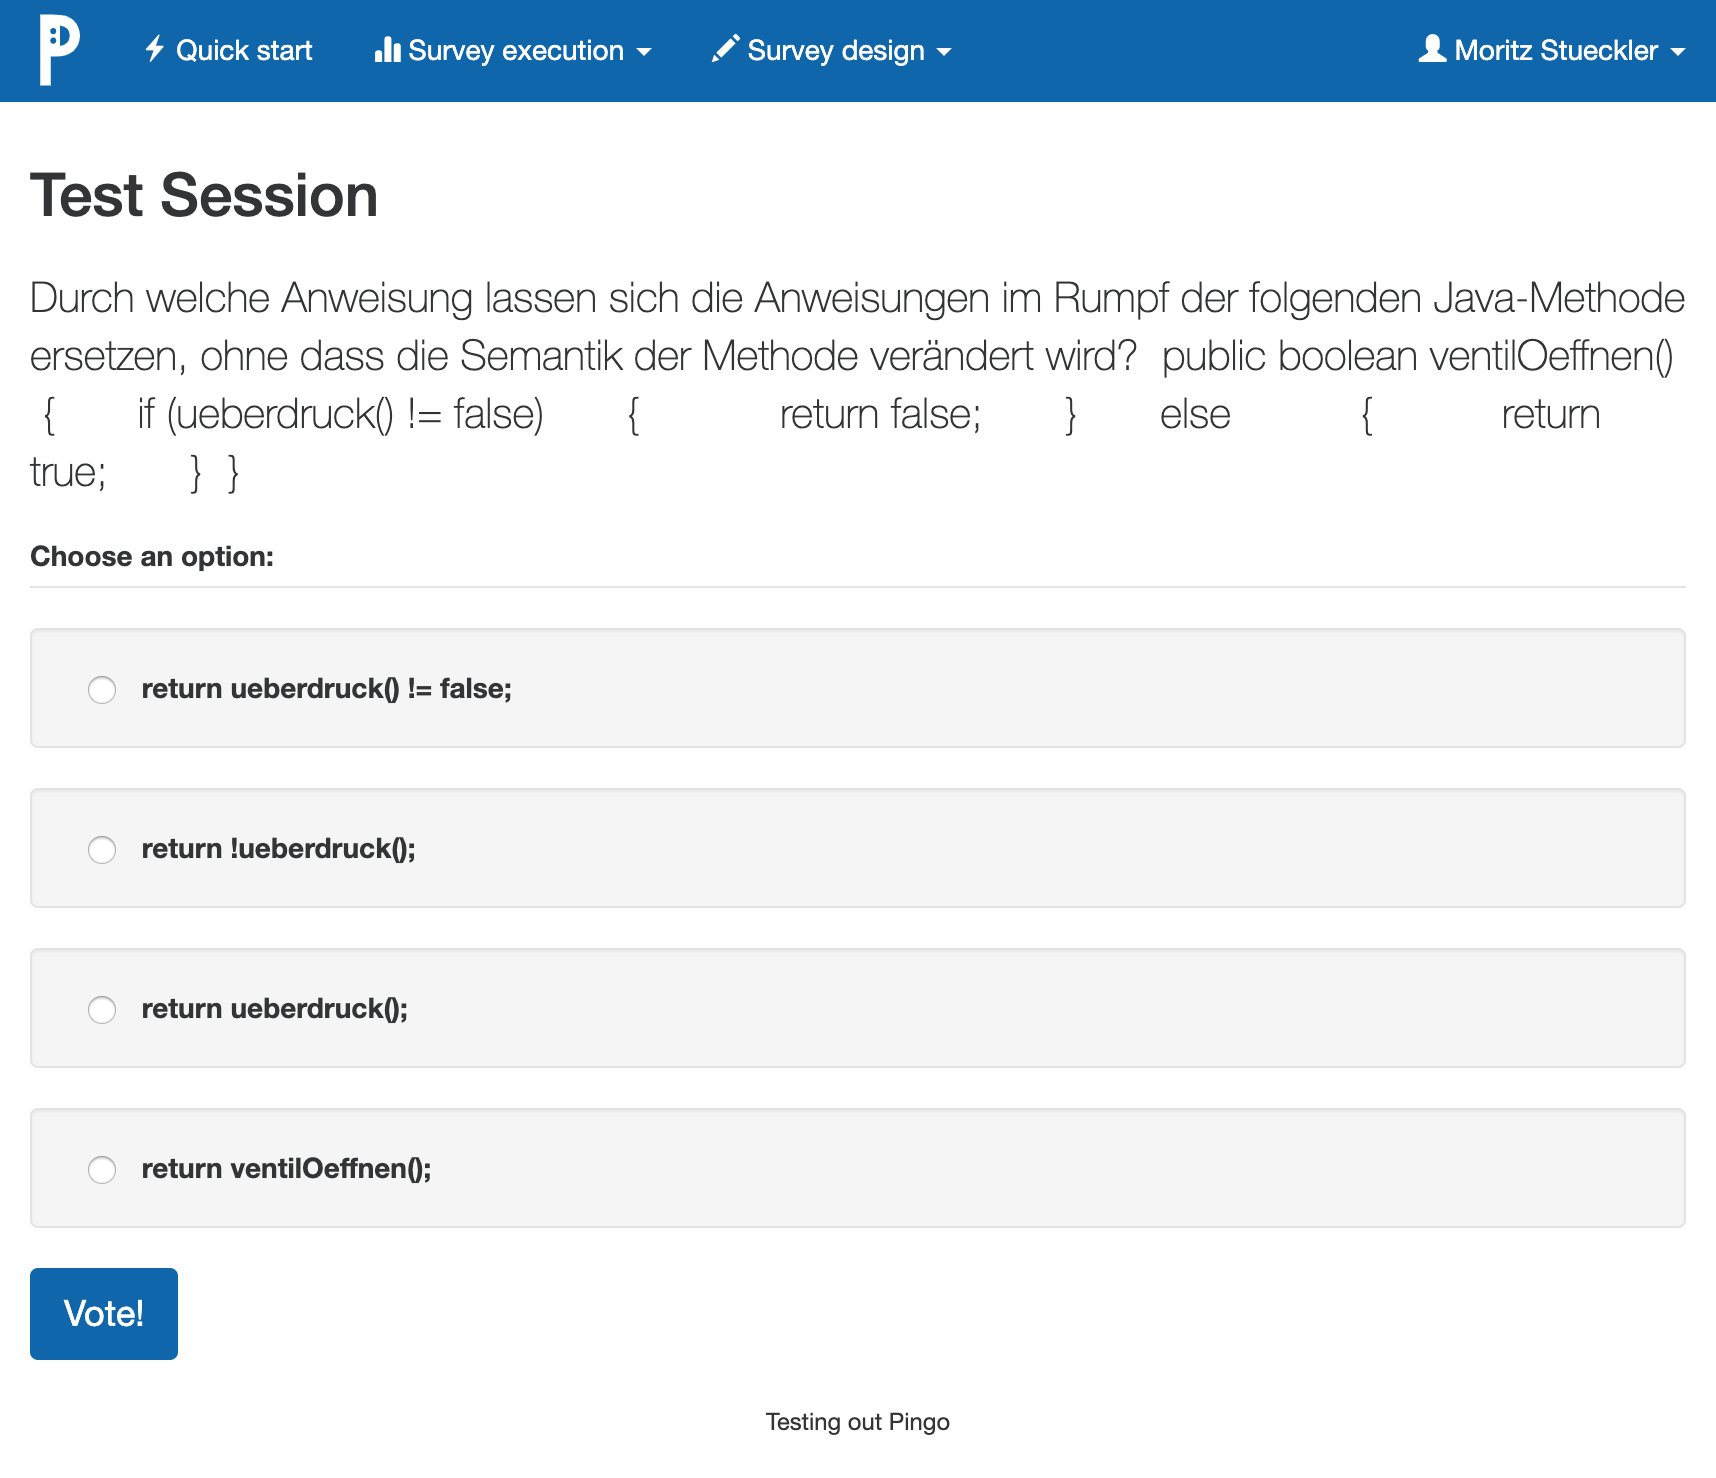
\includegraphics[width=12cm]{chapter/bewertung/bilder/pingo_problem1.png}
    \centering
    \caption{Pingo verfügt über keinerlei Text-Formatierungsoptionen und ist daher ungeeignet für die Darstellung von Quelltext.}
    \label{Abbildung 2.5}
\end{figure}